% !TeX TXS-program:bibliography = txs:///biber
\documentclass[14pt, russian]{scrartcl}
\let\counterwithout\relax
\let\counterwithin\relax
%\usepackage{lmodern}
\usepackage{float}
\usepackage{xcolor}
\usepackage{extsizes}
\usepackage{subfig}
\usepackage[export]{adjustbox}
\usepackage{tocvsec2} % возможность менять учитываемую глубину разделов в оглавлении
\usepackage[subfigure]{tocloft}
\usepackage[newfloat]{minted}
\captionsetup[listing]{position=top}

\AtBeginEnvironment{figure}{\vspace{0.5cm}}
\AtBeginEnvironment{table}{\vspace{0.5cm}}
\AtBeginEnvironment{listing}{\vspace{0.5cm}}
\AtBeginEnvironment{algorithm}{\vspace{0.5cm}}
\AtBeginEnvironment{minted}{\vspace{-0.5cm}}

\usepackage{fancyvrb}
\usepackage{ulem,bm,mathrsfs,ifsym} %зачеркивания, особо жирный стиль и RSFS начертание
\usepackage{sectsty} % переопределение стилей подразделов
%%%%%%%%%%%%%%%%%%%%%%%

%%% Поля и разметка страницы %%%
\usepackage{pdflscape}                              % Для включения альбомных страниц
\usepackage{geometry}                               % Для последующего задания полей
\geometry{a4paper,tmargin=2cm,bmargin=2cm,lmargin=3cm,rmargin=1cm} % тоже самое, но лучше

%%% Математические пакеты %%%
\usepackage{amsthm,amsfonts,amsmath,amssymb,amscd}  % Математические дополнения от AMS
\usepackage{mathtools}                              % Добавляет окружение multlined
\usepackage[perpage]{footmisc}
%\usepackage{times}

%%%% Установки для размера шрифта 14 pt %%%%
%% Формирование переменных и констант для сравнения (один раз для всех подключаемых файлов)%%
%% должно располагаться до вызова пакета fontspec или polyglossia, потому что они сбивают его работу
%\newlength{\curtextsize}
%\newlength{\bigtextsize}
%\setlength{\bigtextsize}{13pt}
\KOMAoptions{fontsize=14pt}

\makeatletter
\def\showfontsize{\f@size{} point}
\makeatother

%\makeatletter
%\show\f@size                                       % неплохо для отслеживания, но вызывает стопорение процесса, если документ компилируется без команды  -interaction=nonstopmode 
%\setlength{\curtextsize}{\f@size pt}
%\makeatother

%шрифт times
\usepackage{tempora}
%\usepackage{pscyr}
%\setmainfont[Ligatures={TeX,Historic}]{Times New Roman}

   %%% Решение проблемы копирования текста в буфер кракозябрами
%    \input glyphtounicode.tex
%    \input glyphtounicode-cmr.tex %from pdfx package
%    \pdfgentounicode=1
    \usepackage{cmap}                               % Улучшенный поиск русских слов в полученном pdf-файле
    \usepackage[T1]{fontenc}                       % Поддержка русских букв
    \usepackage[utf8]{inputenc}                     % Кодировка utf8
    \usepackage[english, main=russian]{babel}            % Языки: русский, английский
%   \IfFileExists{pscyr.sty}{\usepackage{pscyr}}{}  % Красивые русские шрифты
%\renewcommand{\rmdefault}{ftm}
%%% Оформление абзацев %%%
\usepackage{indentfirst}                            % Красная строка
%\usepackage{eskdpz}

%%% Таблицы %%%
\usepackage{longtable}                              % Длинные таблицы
\usepackage{multirow,makecell,array}                % Улучшенное форматирование таблиц
\usepackage{booktabs}                               % Возможность оформления таблиц в классическом книжном стиле (при правильном использовании не противоречит ГОСТ)

%%% Общее форматирование
\usepackage{soulutf8}                               % Поддержка переносоустойчивых подчёркиваний и зачёркиваний
\usepackage{icomma}                                 % Запятая в десятичных дробях



%%% Изображения %%%
\usepackage{graphicx}                               % Подключаем пакет работы с графикой
\usepackage{wrapfig}

%%% Списки %%%
\usepackage{enumitem}

%%% Подписи %%%
\usepackage{caption}                                % Для управления подписями (рисунков и таблиц) % Может управлять номерами рисунков и таблиц с caption %Иногда может управлять заголовками в списках рисунков и таблиц
%% Использование:
%\begin{table}[h!]\ContinuedFloat - чтобы не переключать счетчик
%\captionsetup{labelformat=continued}% должен стоять до самого caption
%\caption{}
% либо ручками \caption*{Продолжение таблицы~\ref{...}.} :)

%%% Интервалы %%%
\addto\captionsrussian{%
  \renewcommand{\listingname}{Листинг}%
}
%%% Счётчики %%%
\usepackage[figure,table,section]{totalcount}               % Счётчик рисунков и таблиц
\DeclareTotalCounter{lstlisting}
\usepackage{totcount}                               % Пакет создания счётчиков на основе последнего номера подсчитываемого элемента (может требовать дважды компилировать документ)
\usepackage{totpages}                               % Счётчик страниц, совместимый с hyperref (ссылается на номер последней страницы). Желательно ставить последним пакетом в преамбуле

%%% Продвинутое управление групповыми ссылками (пока только формулами) %%%
%% Кодировки и шрифты %%%

%   \newfontfamily{\cyrillicfont}{Times New Roman}
%   \newfontfamily{\cyrillicfonttt}{CMU Typewriter Text}
	%\setmainfont{Times New Roman}
	%\newfontfamily\cyrillicfont{Times New Roman}
	%\setsansfont{Times New Roman}                    %% задаёт шрифт без засечек
%	\setmonofont{Liberation Mono}               %% задаёт моноширинный шрифт
%    \IfFileExists{pscyr.sty}{\renewcommand{\rmdefault}{ftm}}{}
%%% Интервалы %%%
%linespread-реализация ближе к реализации полуторного интервала в ворде.
%setspace реализация заточена под шрифты 10, 11, 12pt, под остальные кегли хуже, но всё же ближе к типографской классике. 
\linespread{1.3}                    % Полуторный интервал (ГОСТ Р 7.0.11-2011, 5.3.6)
%\renewcommand{\@biblabel}[1]{#1}

%%% Гиперссылки %%%
\usepackage{hyperref}

%%% Выравнивание и переносы %%%
\sloppy                             % Избавляемся от переполнений
\clubpenalty=10000                  % Запрещаем разрыв страницы после первой строки абзаца
\widowpenalty=10000                 % Запрещаем разрыв страницы после последней строки абзаца

\makeatletter % малые заглавные, small caps shape
\let\@@scshape=\scshape
\renewcommand{\scshape}{%
  \ifnum\strcmp{\f@series}{bx}=\z@
    \usefont{T1}{cmr}{bx}{sc}%
  \else
    \ifnum\strcmp{\f@shape}{it}=\z@
      \fontshape{scsl}\selectfont
    \else
      \@@scshape
    \fi
  \fi}
\makeatother

%%% Подписи %%%
%\captionsetup{%
%singlelinecheck=off,                % Многострочные подписи, например у таблиц
%skip=2pt,                           % Вертикальная отбивка между подписью и содержимым рисунка или таблицы определяется ключом
%justification=centering,            % Центрирование подписей, заданных командой \caption
%}
%%%        Подключение пакетов                 %%%
\usepackage{ifthen}                 % добавляет ifthenelse
%%% Инициализирование переменных, не трогать!  %%%
\newcounter{intvl}
\newcounter{otstup}
\newcounter{contnumeq}
\newcounter{contnumfig}
\newcounter{contnumtab}
\newcounter{pgnum}
\newcounter{bibliosel}
\newcounter{chapstyle}
\newcounter{headingdelim}
\newcounter{headingalign}
\newcounter{headingsize}
\newcounter{tabcap}
\newcounter{tablaba}
\newcounter{tabtita}
%%%%%%%%%%%%%%%%%%%%%%%%%%%%%%%%%%%%%%%%%%%%%%%%%%

%%% Область упрощённого управления оформлением %%%

%% Интервал между заголовками и между заголовком и текстом
% Заголовки отделяют от текста сверху и снизу тремя интервалами (ГОСТ Р 7.0.11-2011, 5.3.5)
\setcounter{intvl}{3}               % Коэффициент кратности к размеру шрифта

%% Отступы у заголовков в тексте
\setcounter{otstup}{0}              % 0 --- без отступа; 1 --- абзацный отступ

%% Нумерация формул, таблиц и рисунков
\setcounter{contnumeq}{1}           % Нумерация формул: 0 --- пораздельно (во введении подряд, без номера раздела); 1 --- сквозная нумерация по всей диссертации
\setcounter{contnumfig}{1}          % Нумерация рисунков: 0 --- пораздельно (во введении подряд, без номера раздела); 1 --- сквозная нумерация по всей диссертации
\setcounter{contnumtab}{1}          % Нумерация таблиц: 0 --- пораздельно (во введении подряд, без номера раздела); 1 --- сквозная нумерация по всей диссертации

%% Оглавление
\setcounter{pgnum}{0}               % 0 --- номера страниц никак не обозначены; 1 --- Стр. над номерами страниц (дважды компилировать после изменения)

%% Библиография
\setcounter{bibliosel}{1}           % 0 --- встроенная реализация с загрузкой файла через движок bibtex8; 1 --- реализация пакетом biblatex через движок biber

%% Текст и форматирование заголовков
\setcounter{chapstyle}{1}           % 0 --- разделы только под номером; 1 --- разделы с названием "Глава" перед номером
\setcounter{headingdelim}{1}        % 0 --- номер отделен пропуском в 1em или \quad; 1 --- номера разделов и приложений отделены точкой с пробелом, подразделы пропуском без точки; 2 --- номера разделов, подразделов и приложений отделены точкой с пробелом.

%% Выравнивание заголовков в тексте
\setcounter{headingalign}{0}        % 0 --- по центру; 1 --- по левому краю

%% Размеры заголовков в тексте
\setcounter{headingsize}{0}         % 0 --- по ГОСТ, все всегда 14 пт; 1 --- пропорционально изменяющийся размер в зависимости от базового шрифта

%% Подпись таблиц
\setcounter{tabcap}{0}              % 0 --- по ГОСТ, номер таблицы и название разделены тире, выровнены по левому краю, при необходимости на нескольких строках; 1 --- подпись таблицы не по ГОСТ, на двух и более строках, дальнейшие настройки: 
%Выравнивание первой строки, с подписью и номером
\setcounter{tablaba}{2}             % 0 --- по левому краю; 1 --- по центру; 2 --- по правому краю
%Выравнивание строк с самим названием таблицы
\setcounter{tabtita}{1}             % 0 --- по левому краю; 1 --- по центру; 2 --- по правому краю

%%% Рисунки %%%
\DeclareCaptionLabelSeparator*{emdash}{~--- }             % (ГОСТ 2.105, 4.3.1)
\captionsetup[figure]{labelsep=emdash,font=onehalfspacing,position=bottom}

%%% Таблицы %%%
\ifthenelse{\equal{\thetabcap}{0}}{%
    \newcommand{\tabcapalign}{\raggedright}  % по левому краю страницы или аналога parbox
}

\ifthenelse{\equal{\thetablaba}{0} \AND \equal{\thetabcap}{1}}{%
    \newcommand{\tabcapalign}{\raggedright}  % по левому краю страницы или аналога parbox
}

\ifthenelse{\equal{\thetablaba}{1} \AND \equal{\thetabcap}{1}}{%
    \newcommand{\tabcapalign}{\centering}    % по центру страницы или аналога parbox
}

\ifthenelse{\equal{\thetablaba}{2} \AND \equal{\thetabcap}{1}}{%
    \newcommand{\tabcapalign}{\raggedleft}   % по правому краю страницы или аналога parbox
}

\ifthenelse{\equal{\thetabtita}{0} \AND \equal{\thetabcap}{1}}{%
    \newcommand{\tabtitalign}{\raggedright}  % по левому краю страницы или аналога parbox
}

\ifthenelse{\equal{\thetabtita}{1} \AND \equal{\thetabcap}{1}}{%
    \newcommand{\tabtitalign}{\centering}    % по центру страницы или аналога parbox
}

\ifthenelse{\equal{\thetabtita}{2} \AND \equal{\thetabcap}{1}}{%
    \newcommand{\tabtitalign}{\raggedleft}   % по правому краю страницы или аналога parbox
}

\DeclareCaptionFormat{tablenocaption}{\tabcapalign #1\strut}        % Наименование таблицы отсутствует
\ifthenelse{\equal{\thetabcap}{0}}{%
    \DeclareCaptionFormat{tablecaption}{\tabcapalign #1#2#3}
    \captionsetup[table]{labelsep=emdash}                       % тире как разделитель идентификатора с номером от наименования
}{%
    \DeclareCaptionFormat{tablecaption}{\tabcapalign #1#2\par%  % Идентификатор таблицы на отдельной строке
        \tabtitalign{#3}}                                       % Наименование таблицы строкой ниже
    \captionsetup[table]{labelsep=space}                        % пробельный разделитель идентификатора с номером от наименования
}
\captionsetup[table]{format=tablecaption,singlelinecheck=off,font=onehalfspacing,position=top,skip=-5pt}  % многострочные наименования и прочее
\DeclareCaptionLabelFormat{continued}{Продолжение таблицы~#2}
\setlength{\belowcaptionskip}{.2cm}
\setlength{\intextsep}{0ex}

%%% Подписи подрисунков %%%
\renewcommand{\thesubfigure}{\asbuk{subfigure}}           % Буквенные номера подрисунков
\captionsetup[subfigure]{font={normalsize},               % Шрифт подписи названий подрисунков (не отличается от основного)
    labelformat=brace,                                    % Формат обозначения подрисунка
    justification=centering,                              % Выключка подписей (форматирование), один из вариантов            
}
%\DeclareCaptionFont{font12pt}{\fontsize{12pt}{13pt}\selectfont} % объявляем шрифт 12pt для использования в подписях, тут же надо интерлиньяж объявлять, если не наследуется
%\captionsetup[subfigure]{font={font12pt}}                 % Шрифт подписи названий подрисунков (всегда 12pt)

%%% Настройки гиперссылок %%%

\definecolor{linkcolor}{rgb}{0.0,0,0}
\definecolor{citecolor}{rgb}{0,0.0,0}
\definecolor{urlcolor}{rgb}{0,0,0}

\hypersetup{
    linktocpage=true,           % ссылки с номера страницы в оглавлении, списке таблиц и списке рисунков
%    linktoc=all,                % both the section and page part are links
%    pdfpagelabels=false,        % set PDF page labels (true|false)
    plainpages=true,           % Forces page anchors to be named by the Arabic form  of the page number, rather than the formatted form
    colorlinks,                 % ссылки отображаются раскрашенным текстом, а не раскрашенным прямоугольником, вокруг текста
    linkcolor={linkcolor},      % цвет ссылок типа ref, eqref и подобных
    citecolor={citecolor},      % цвет ссылок-цитат
    urlcolor={urlcolor},        % цвет гиперссылок
    pdflang={ru},
}
\urlstyle{same}
%%% Шаблон %%%
%\DeclareRobustCommand{\todo}{\textcolor{red}}       % решаем проблему превращения названия цвета в результате \MakeUppercase, http://tex.stackexchange.com/a/187930/79756 , \DeclareRobustCommand protects \todo from expanding inside \MakeUppercase
\setlength{\parindent}{2.5em}                       % Абзацный отступ. Должен быть одинаковым по всему тексту и равен пяти знакам (ГОСТ Р 7.0.11-2011, 5.3.7).

%%% Списки %%%
% Используем дефис для ненумерованных списков (ГОСТ 2.105-95, 4.1.7)
%\renewcommand{\labelitemi}{\normalfont\bfseries~{---}} 
\renewcommand{\labelitemi}{\bfseries~{---}} 
\setlist{nosep,%                                    % Единый стиль для всех списков (пакет enumitem), без дополнительных интервалов.
    labelindent=\parindent,leftmargin=*%            % Каждый пункт, подпункт и перечисление записывают с абзацного отступа (ГОСТ 2.105-95, 4.1.8)
}
%%%%%%%%%%%%%%%%%%%%%%
%\usepackage{xltxtra} % load xunicode

\usepackage{ragged2e}
\usepackage[explicit]{titlesec}
\usepackage{placeins}
\usepackage{xparse}
\usepackage{csquotes}

\usepackage{listingsutf8}
\usepackage{url} %пакеты расширений
\usepackage{algorithm, algorithmicx}
\usepackage[noend]{algpseudocode}
\usepackage{blkarray}
\usepackage{chngcntr}
\usepackage{tabularx}
\usepackage[backend=biber, 
    bibstyle=gost-numeric,
    citestyle=nature]{biblatex}
\newcommand*\template[1]{\text{<}#1\text{>}}
\addbibresource{biblio.bib}
  
\titleformat{name=\section,numberless}[block]{\normalfont\Large\centering}{}{0em}{#1}
\titleformat{\section}[block]{\normalfont\Large\bfseries\raggedright}{}{0em}{\thesection\hspace{0.25em}#1}
\titleformat{\subsection}[block]{\normalfont\Large\bfseries\raggedright}{}{0em}{\thesubsection\hspace{0.25em}#1}
\titleformat{\subsubsection}[block]{\normalfont\large\bfseries\raggedright}{}{0em}{\thesubsubsection\hspace{0.25em}#1}

\let\Algorithm\algorithm
\renewcommand\algorithm[1][]{\Algorithm[#1]\setstretch{1.5}}
%\renewcommand{\listingscaption}{Листинг}

\usepackage{pifont}
\usepackage{calc}
\usepackage{suffix}
\usepackage{csquotes}
\DeclareQuoteStyle{russian}
    {\guillemotleft}{\guillemotright}[0.025em]
    {\quotedblbase}{\textquotedblleft}
\ExecuteQuoteOptions{style=russian}
\newcommand{\enq}[1]{\enquote{#1}}  
\newcommand{\eng}[1]{\begin{english}#1\end{english}}
% Подчиненные счетчики в окружениях http://old.kpfu.ru/journals/izv_vuz/arch/sample1251.tex
\newcounter{cTheorem} 
\newcounter{cDefinition}
\newcounter{cConsequent}
\newcounter{cExample}
\newcounter{cLemma}
\newcounter{cConjecture}
\newtheorem{Theorem}{Теорема}[cTheorem]
\newtheorem{Definition}{Определение}[cDefinition]
\newtheorem{Consequent}{Следствие}[cConsequent]
\newtheorem{Example}{Пример}[cExample]
\newtheorem{Lemma}{Лемма}[cLemma]
\newtheorem{Conjecture}{Гипотеза}[cConjecture]

\renewcommand{\theTheorem}{\arabic{Theorem}}
\renewcommand{\theDefinition}{\arabic{Definition}}
\renewcommand{\theConsequent}{\arabic{Consequent}}
\renewcommand{\theExample}{\arabic{Example}}
\renewcommand{\theLemma}{\arabic{Lemma}}
\renewcommand{\theConjecture}{\arabic{Conjecture}}
%\makeatletter
\NewDocumentCommand{\Newline}{}{\text{\\}}
\newcommand{\sequence}[2]{\ensuremath \left(#1,\ \dots,\ #2\right)}

\definecolor{mygreen}{rgb}{0,0.6,0}
\definecolor{mygray}{rgb}{0.5,0.5,0.5}
\definecolor{mymauve}{rgb}{0.58,0,0.82}
\renewcommand{\listalgorithmname}{Список алгоритмов}
\floatname{algorithm}{Листинг}
\renewcommand{\lstlistingname}{Листинг}
\renewcommand{\thealgorithm}{\arabic{algorithm}}

\newcommand{\refAlgo}[1]{(листинг \ref{#1})}
\newcommand{\refImage}[1]{(рисунок \ref{#1})}

\renewcommand{\theenumi}{\arabic{enumi}.}% Меняем везде перечисления на цифра.цифра	
\renewcommand{\labelenumi}{\arabic{enumi}.}% Меняем везде перечисления на цифра.цифра
\renewcommand{\theenumii}{\arabic{enumii}}% Меняем везде перечисления на цифра.цифра
\renewcommand{\labelenumii}{(\arabic{enumii})}% Меняем везде перечисления на цифра.цифра
\renewcommand{\theenumiii}{\roman{enumiii}}% Меняем везде перечисления на цифра.цифра
\renewcommand{\labelenumiii}{(\roman{enumiii})}% Меняем везде перечисления на цифра.цифра
%\newfontfamily\AnkaCoder[Path=src/fonts/]{AnkaCoder-r.ttf}
\renewcommand{\labelitemi}{---}
\renewcommand{\labelitemii}{---}

%\usepackage{courier}

\lstdefinelanguage{Refal}{
  alsodigit = {.,<,>},
  morekeywords = [1]{$ENTRY},
  morekeywords = [2]{Go, Put, Get, Open, Close, Arg, Add, Sub, Mul, Div, Symb, Explode, Implode},
  %keyword4
  morekeywords = [3]{<,>},
  %keyword5
  morekeywords = [4]{e.,t.,s.},
  sensitive = true,
  morecomment = [l]{*},
  morecomment = [s]{/*}{*/},
  commentstyle = \color{mygreen},
  morestring = [b]",
  morestring = [b]',
  stringstyle = \color{purple}
}

\makeatletter
\def\p@subsection{}
\def\p@subsubsection{\thesection\,\thesubsection\,}
\makeatother
\newcommand{\prog}[1]{{\ttfamily\small#1}}
\lstset{ %
  backgroundcolor=\color{white},   % choose the background color; you must add \usepackage{color} or \usepackage{xcolor}
  basicstyle=\ttfamily\footnotesize, 
  %basicstyle=\footnotesize\AnkaCoder,        % the size of the fonts that are used for the code
  breakatwhitespace=false,         % sets if automatic breaks shoulbd only happen at whitespace
  breaklines=true,                 % sets automatic line breaking
  captionpos=top,                    % sets the caption-position to bottom
  commentstyle=\color{mygreen},    % comment style
  deletekeywords={...},            % if you want to delete keywords from the given language
  escapeinside={\%*}{*)},          % if you want to add LaTeX within your code
  extendedchars=true,              % lets you use non-ASCII characters; for 8-bits encodings only, does not work with UTF-8
  inputencoding=utf8,
  frame=single,                    % adds a frame around the code
  keepspaces=true,                 % keeps spaces in text, useful for keeping indentation of code (possibly needs columns=flexible)
  keywordstyle=\bf,       % keyword style
  language=Refal,                    % the language of the code
  morekeywords={<,>,$ENTRY,Go,Arg, Open, Close, e., s., t., Get, Put}, 
  							       % if you want to add more keywords to the set
  numbers=left,                    % where to put the line-numbers; possible values are (none, left, right)
  numbersep=5pt,                   % how far the line-numbers are from the code
  xleftmargin=25pt,
  xrightmargin=25pt,
  numberstyle=\small\color{black}, % the style that is used for the line-numbers
  rulecolor=\color{black},         % if not set, the frame-color may be changed on line-breaks within not-black text (e.g. comments (green here))
  showspaces=false,                % show spaces everywhere adding particular underscores; it overrides 'showstringspaces'
  showstringspaces=false,          % underline spaces within strings only
  showtabs=false,                  % show tabs within strings adding particular underscores
  stepnumber=1,                    % the step between two line-numbers. If it's 1, each line will be numbered
  stringstyle=\color{mymauve},     % string literal style
  tabsize=8,                       % sets default tabsize to 8 spaces
  title=\lstname                   % show the filename of files included with \lstinputlisting; also try caption instead of title
}
\newcommand{\anonsection}[1]{\cleardoublepage
\phantomsection
\addcontentsline{toc}{section}{\protect\numberline{}#1}
\section*{#1}\vspace*{2.5ex} % По госту положены 3 пустые строки после заголовка ненумеруемого раздела
}
\newcommand{\sectionbreak}{\clearpage}
\renewcommand{\sectionfont}{\normalsize} % Сбиваем стиль оглавления в стандартный
\renewcommand{\cftsecleader}{\cftdotfill{\cftdotsep}} % Точки в оглавлении напротив разделов

\renewcommand{\cftsecfont}{\normalfont\large} % Переключение на times в содержании
\renewcommand{\cftsubsecfont}{\normalfont\large} % Переключение на times в содержании

\usepackage{caption} 
%\captionsetup[table]{justification=raggedleft} 
%\captionsetup[figure]{justification=centering,labelsep=endash}
\usepackage{amsmath}    % \bar    (матрицы и проч. ...)
\usepackage{amsfonts}   % \mathbb (символ для множества действительных чисел и проч. ...)
\usepackage{mathtools}  % \abs, \norm
    \DeclarePairedDelimiter\abs{\lvert}{\rvert} % операция модуля
    \DeclarePairedDelimiter\norm{\lVert}{\rVert} % операция нормы
\DeclareTextCommandDefault{\textvisiblespace}{%
  \mbox{\kern.06em\vrule \@height.3ex}%
  \vbox{\hrule \@width.3em}%
  \hbox{\vrule \@height.3ex}}    
\newsavebox{\spacebox}
\begin{lrbox}{\spacebox}
\verb*! !
\end{lrbox}
\newcommand{\aspace}{\usebox{\spacebox}}
\DeclareTotalCounter{listing}

\makeatletter
\renewcommand*{\p@subsubsection}{}
\makeatother
    
\begin{document}
\sloppy

\def\figurename{Рисунок}

\begin{titlepage}
\thispagestyle{empty}
\newpage

\vspace*{-30pt}
\hspace{-45pt}
\begin{minipage}{0.17\textwidth}
\hspace*{-20pt}\centering
\includegraphics[width=1.3\textwidth]{emblem.png}
\end{minipage}
\begin{minipage}{0.82\textwidth}\small \textbf{
\vspace*{-0.7ex}
\hspace*{-10pt}\centerline{Министерство науки и высшего образования Российской Федерации}
\vspace*{-0.7ex}
\centerline{Федеральное государственное бюджетное образовательное учреждение }
\vspace*{-0.7ex}
\centerline{высшего образования}
\vspace*{-0.7ex}
\centerline{<<Московский государственный технический университет}
\vspace*{-0.7ex}
\centerline{имени Н.Э. Баумана}
\vspace*{-0.7ex}
\centerline{(национальный исследовательский университет)>>}
\vspace*{-0.7ex}
\centerline{(МГТУ им. Н.Э. Баумана)}}
\end{minipage}

\vspace{-2pt}
\hspace{-34.5pt}\rule{\textwidth}{2.5pt}

\vspace*{-20.3pt}
\hspace{-34.5pt}\rule{\textwidth}{0.4pt}
 
\vspace{0.5ex}
\noindent \small ФАКУЛЬТЕТ\hspace{80pt} <<Информатика и системы управления>>

\vspace*{-16pt}
\hspace{35pt}\rule{0.855\textwidth}{0.4pt}

\vspace{0.5ex}
\noindent \small КАФЕДРА\hspace{50pt} <<Теоретическая информатика и компьютерные технологии>>

\vspace*{-16pt}
\hspace{25pt}\rule{0.875\textwidth}{0.4pt}
 
 
\vspace{3em}
 
\begin{center}
\Large \bf{РАСЧЕТНО-ПОЯСНИТЕЛЬНАЯ ЗАПИСКА\\\textbf{\textit{К КУРСОВОЙ РАБОТЕ\\НА ТЕМУ:}} \\}
\end{center}

\vspace*{-6ex} 
\begin{center}
\Large{\textit{\textbf{<<Визуализация графа связей пользователей }}}

\vspace*{-3ex}
\rule{0.9\textwidth}{1.2pt}

\vspace*{-0.2ex}
\Large{\textit{\textbf{социальной сети>>}}}
\vspace*{-3ex}
\vspace*{-0.2ex}
\rule{0.9\textwidth}{1.2pt}

\vspace*{-0.2ex}
\rule{0.9\textwidth}{1.2pt}

\vspace*{-0.2ex}
\rule{0.9\textwidth}{1.2pt}

\vspace*{-0.2ex}
\rule{0.9\textwidth}{1.2pt}
\end{center}
 
\vspace{\fill}
 

\newlength{\ML}
\settowidth{\ML}{«\underline{\hspace{0.7cm}}» \underline{\hspace{2cm}}}

\noindent Студент \underline{\text{ИУ9-51Б}} \hfill \underline{ \hspace{4cm}}\quad
\underline{\parbox{4cm}{\centering Киселев К.А.}}

\vspace{-2.1ex}
\noindent\hspace{9ex}\scriptsize{(Группа)}\normalsize\hspace{170pt}\hspace{2ex}\scriptsize{(Подпись, дата)}\normalsize\hspace{30pt}\hspace{6ex}\scriptsize{(И.О. Фамилия)}\normalsize

\bigskip

\noindent Руководитель  \hfill \underline{\hspace{4cm}}\quad
\underline{\parbox{4cm}{\centering Каганов Ю.Т.}}

\vspace{-2ex}
\noindent\hspace{13.5ex}\normalsize\hspace{170pt}\hspace{2ex}\scriptsize{(Подпись, дата)}\normalsize\hspace{30pt}\hspace{6ex}\scriptsize{(И.О. Фамилия)}\normalsize

\bigskip

\noindent Консультант\hfill \underline{\hspace{4cm}}\quad
\underline{\hspace{4cm}}

\vspace{-2ex}
\noindent\hspace{13.5ex}\normalsize\hspace{170pt}\hspace{2ex}\scriptsize{(Подпись, дата)}\normalsize\hspace{30pt}\hspace{6ex}\scriptsize{(И.О. Фамилия)}\normalsize
\vfill

%\vspace{\fill}
 


\begin{center}
\textsl{2023 г.}
\end{center}
\end{titlepage}

%\renewcommand{\ttdefault}{pcr}

\setlength{\tabcolsep}{3pt}
\newpage
\setcounter{page}{2}
%----------------------------------------------------------------------------
%                  ОТСЮДА --- СОБСТВЕННО ТЕКСТ
%----------------------------------------------------------------------------

\newpage
\renewcommand\contentsname{\hfill{\normalfont{СОДЕРЖАНИЕ}}\hfill}  %Оглавление
\tableofcontents
\newpage
\anonsection{ВВЕДЕНИЕ}  %Введение

В эпоху цифровых коммуникаций социальные сети играют ключевую роль в повседневной жизни, предоставляя своим пользователям возможность активного взаимодействия и обмена информацией.
С ростом объема данных, сгенерированных социальными платформами, возникает неотложная потребность в разработке эффективных методов анализа, позволяющих понять сложные взаимосвязи между участниками сети. В данном контексте визуализация связей пользователей становится ключевым инструментом, обеспечивающим наглядное отображение структуры социальных взаимодействий.

Целью данной курсовой работы является разработка программы для
визуализации данных о связях пользователей социальной сети на основе графовой модели.

\section{Обзор предметной области}

Связи пользователей социальной сети естественным образом представляются с помощью графовой модели,
где вершинами являются пользователи, а ребрами --- связи между ними (например, <<дружба>> и т.д.).
Пригодное для анализа представление должно удовлетворять следующим критериям:

\begin{itemize}
	\item Минимимальность пересечений ребер;
	\item Равномерность распределение вершин; 
	\item Однородность длин ребер; 
	\item Наличие симметрии.
\end{itemize}

Силовые алгоритмы визуализации графов представляют собой класс алгоритмов, цель которых заключается в улучшении эстетических характеристик графического представления.
Основной задачей этих алгоритмов является такое размещение узлов графа в двухмерном или трехмерном пространстве, чтобы длины рёбер были приблизительно одинаковыми,
и при этом количество пересечений рёбер было минимальным.
Пример визуализации графа связей статей на Wikipedia, полученной с помощью силового алгоритма изображен на рисунке \ref{fig:force_directed_example} 


\begin{figure}[H]
\centering
  \begin{minipage}[t]{.8\textwidth}
  \centering
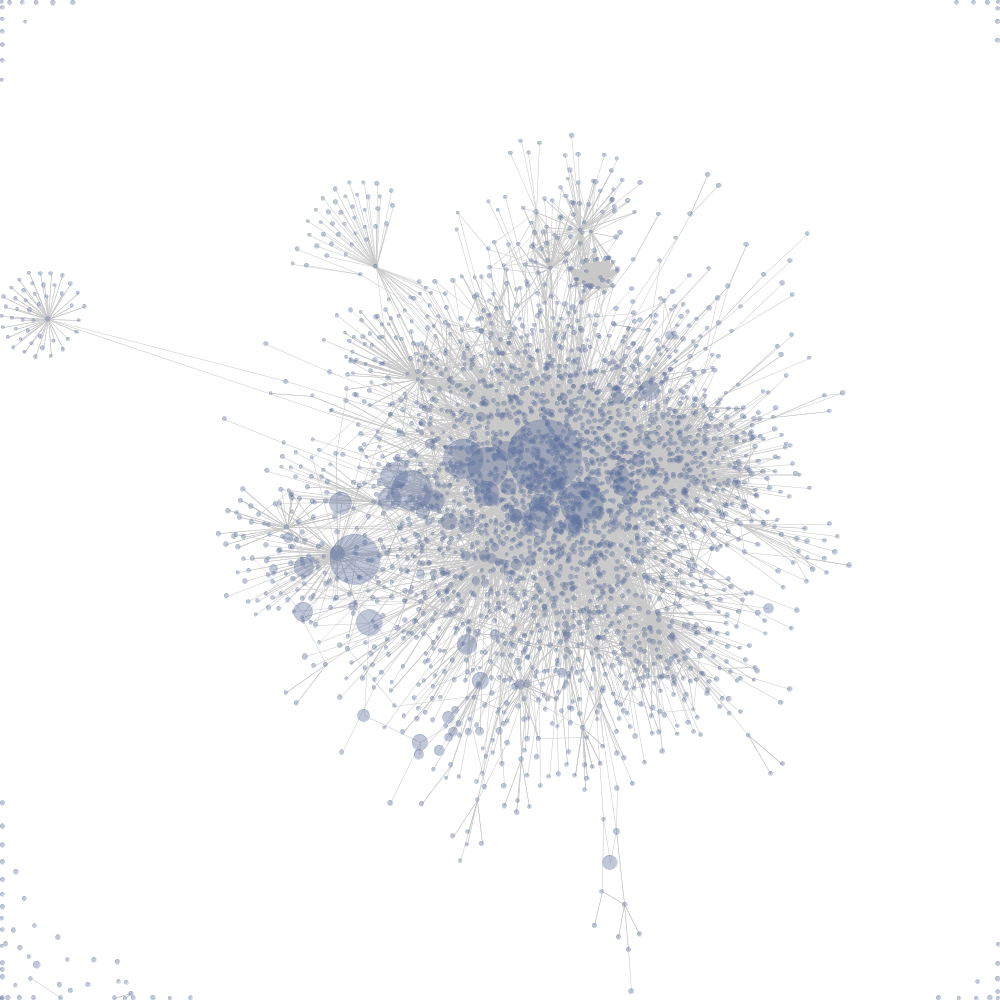
\includegraphics[width=.7\textwidth]{./imgs/force-directed-example.png}
  \end{minipage}
\caption{Визуализация графа с помощью силового алгоритма.}
\label{fig:force_directed_example}
\end{figure}

\subsection{Силовые алгоритмы}

Силовые алгоритмы визуализации графов оперируют основными принципами сил и энергии в физическом смысле, чтобы достичь оптимального распределения узлов и рёбер в графе.

Основные этапы и принципы их работы:

\begin{enumerate}
	\item Инициализация. Начальное распределение узлов графа задаётся случайным образом или с использованием предварительных координат;
	\item Определение сил. Алгоритм вычисляет силы для каждого узла, основываясь на их текущих относительных положениях.
	\item Обновление координат. На основе вычисленных сил происходит обновление координат узлов.
	\item Итерация. Процесс вычисления сил и обновления координат повторяется в циклах, обычно до тех пор, пока не будет достигнута определенная степень стабилизации или заданное количество итераций.
\end{enumerate}

Несмотря на  широкое применение, силовые алгоритмы визуализации графов также имеют свои ограничения и минусы:

\begin{enumerate}
  \item{Чувствительность к начальным условиям: Результаты силовых алгоритмов могут зависеть от начального распределения узлов. Различные начальные условия могут привести к разным конечным визуализациям, что может затруднить воспроизводимость результатов.}
  \item{Зависимость от параметров: Силовые алгоритмы имеют различные параметры, такие как коэффициенты отталкивания и притяжения. Оптимальные значения этих параметров могут зависеть от конкретного графа, и их настройка может потребовать экспериментов.}
  \item{Проблемы с большими графами:
При визуализации очень больших графов силовые алгоритмы могут потребовать значительных вычислительных ресурсов и времени. Это может сделать их неэффективными для работы с масштабными социальными сетями или другими крупными графовыми структурами.}
\end{enumerate}

Силовые алгоритмы визуализации графов являются подходящим инструментом для задачи визуализации графа связей пользователей социальной сети. Несмотря на некоторые ограничения, такие как чувствительность к начальным условиям и зависимость от параметров, эти алгоритмы обладают важными преимуществами.

Естественное моделирование физических свойств позволяет отразить реальные взаимодействия в социальных сетях.Кроме того, силовые алгоритмы обеспечивают эстетически привлекательные визуализации с равномерным распределением вершин и минимизацией пересечений рёбер.



\subsection{Алгоритм Идеса}

Алгоритм визуализации графов, разработанный Питером Идесом, представляет собой метод для распределения вершин графа на плоскости таким образом, чтобы минимизировать пересечения рёбер и создать визуально удовлетворительное представление структуры графа. Этот алгоритм был представлен в 1984 году \cite{Eades}.

Каждое ребро графа моделируется как пружина, которая стремится удерживать связанные вершины на определенном расстоянии друг от друга. Если расстояние между вершинами больше желаемого, то действует пружинная сила, направленная на уменьшение расстояния. Если расстояние меньше, то действует отталкивающая сила, направленная на увеличение расстояния. Вершины, не соединенные ребрами, действуют друг на друга отталкивающим образом. Это содействует распределению вершин по плоскости графа, предотвращая их слишком близкое расположение. 

При использовании алгоритма Идеса необходимо определить следующие константы:

\begin{enumerate}
  \item{Число итераций. Это количество итераций, которые алгоритм будет выполнять для уточнения распределения вершин. Большее число итераций может привести к более точной визуализации, но также увеличит вычислительную сложность.}
  \item{Коэффициент жесткоски пружин. Этот коэффициент определяет силу, с которой пружины стремятся удерживать соединенные вершины на определенном расстоянии. Увеличение этого коэффициента сделает пружины более жесткими, а уменьшение — более мягкими.}
  \item{Коэффициент отталкивания. Определяет силу отталкивания между вершинами, которые не соединены ребрами. Увеличение этого коэффициента усиливает силы отталкивания, что приводит к более широкому распределению вершин.}
  \item{Длина пружины. Задает желаемую длину пружины между соединенными вершинами. Этот параметр влияет на силы пружин и, таким образом, на расстояние между вершинами. }
  \item{Шаг обновления. Это значение определяет величину изменения позиции вершин на каждой итерации. Большие значения могут привести к быстрому перемещению вершин, но могут также вызвать колебания и неустойчивость, тогда как малые значения могут сделать процесс слишком медленным.}
\end{enumerate}

Псевдокод алгоритма Идеса представлен на листинге \ref{alg:eades}

\begin{algorithm}[H]
\caption{Алгоритм Идса}\label{alg:eades}
\begin{algorithmic}

  \Function{$f_{spring}$}{$p_u, p_v$}
  \State $r \gets c_{spring}\log{\frac{\|p_v - p_u \|}{l}}  \cdot \overrightarrow{p_u p_v}  $
  
  \Return $r$  
  \EndFunction

 
  \Function{$f_{rep}$}{$p_u, p_v$}
  \State $r \gets \frac{c_{rep}}{\|p_v - p_u \|} \cdot \overrightarrow{p_u p_v}  $
  
  \Return $r$  
  \EndFunction
 

	\Function{Eades}{$G = (V, E)$, $p = (p_{v})_{v \in V}$, $k \in \mathbb{N}$}
	\State $t \gets 1$
	\While{$t \leq K$} 

		\For{$u \in V$}
			\State $F_{u}(t) \gets \sum_{v:\{u,v\} \notin E}{f_{rep}(u, v)} + \sum_{v:\{u,v\} \in E}{f_{spring}(u, v)}$
		

		\EndFor
		\For{$u \in V$}
			\State $p_u \gets p_u + \delta \cdot F_u(t)$
		\EndFor
		
		\State $t \gets t + 1$
	\EndWhile
	\Return $p$
	\EndFunction


\end{algorithmic}
\end{algorithm}



\newpage 

\subsection{Алгоритм Фрюхтермана-Рейнгольда }

Алгоритм Фрюхтермана-Рейнгольда был предложен Томасом Фрюхтерманом и Эдвардом Рейнгольдом в 1991 году \cite{FR}. Этот алгоритм рассматривает вершины графа как <<частицы>>, оказывающие друг на друга притягивающие и  отталкивающие силы. Притягивающие и отталкивающие
силы переопределяются формулами \ref{eq:fr_attractive} и \ref{eq:fr_repulsive} соответственно в терминах расстояния d между двумя вершинами и оптимального расстояния между вершинами, которое определяется формулой \ref{eq:fr_const}


\begin{equation}\label{eq:fr_attractive}
  f_{attr}(d) = \frac{d^2}{k}
\end{equation}

\begin{equation}\label{eq:fr_repulsive}
  f_{rep}(d) = -\frac{k^2}{d}
\end{equation}

\begin{equation}\label{eq:fr_const}
  k = C \sqrt{\frac{width * heigth}{|V|}}
\end{equation} 


Этот алгоритм похож на алгоритм Идеса в том, что оба алгоритма вычисляют притягивающие силы между соседними вершинами и отталкивающие силы между всеми парами вершин.
Алгоритм Фрюхтермана и Рейнгольда добавляет понятие <<температура>>, которое можно использовать следующим образом: <<температура>> может начинаться с начального значения (например, с одной десятой ширины рамки) и убывать до 0 обратным линейным образом. Температура контролирует смещение вершин, так что по мере улучшения компоновки корректировки становятся все меньше. Использование температуры здесь является частным случаем общей техники, называемой имитационным отжигом.

Псевдокод алгоритма Фрюхтермана и Рейнгольда показан на листинге \ref{alg:fr_algorithm}. На каждой итерации базовый алгоритм вычисляет $O(|E|)$ притягивающих сил и $O(|V|^2)$ отталкивающих сил. Чтобы уменьшить квадратичную сложность вычисления отталкивающих сил, Фрюхтерман и Рейнгольд предлагают использовать сеточный вариант своего базового алгоритма, в котором отталкивающие силы между удаленными вершинами игнорируются. Для разреженных графов и при равномерном распределении вершин этот метод позволяет приближенно вычислить силы отталкивания за время $O(|V|)$.


\begin{algorithm}[H]
\caption{Алгоритм Фрюхтермана-Рейнгольда}\label{alg:fr_algorithm}
\begin{algorithmic}

  \Function{$f_{rep}$}{$p_u, p_v$}
  \State $r \gets \frac{l^2}{\|p_v - p_u \|}  \cdot \overrightarrow{p_v p_u}  $
  
  \Return $r$  
  \EndFunction

 
  \Function{$f_{attr}$}{$p_u, p_v$}
  \State $r \gets \frac{\|p_v - p_u \|^2}{l} \cdot \overrightarrow{p_u p_v}  $
  
  \Return $r$  
  \EndFunction
 

	\Function{FruchtermanReingold}{$G = (V, E)$, $p = (p_{v})_{v \in V}$, $k \in \mathbb{N}$}
	\State $t \gets 1$
	\While{$k \leq K$} 

		\For{$u \in V$}
			\State $F_{u}(k) \gets \sum_{v \in V}{f_{rep}(u, v)} + \sum_{v:\{u,v\} \in E}{f_{attr}(u, v)}$
		

		\EndFor
		\For{$u \in V$}
      \State $p_u \gets p_u + \delta(t) \cdot F_u(k)$
		\EndFor
		
    \State $t \gets cool(t)$
		\State $k \gets k + 1$
	\EndWhile
	\Return $p$
	\EndFunction

\end{algorithmic}
\end{algorithm}

Основные шаги алгоритма:

\begin{enumerate}
  \item{Инициализация расположения вершин. Вершины графа случайным образом размещаются в двумерном пространстве;}
  \item{Вычисление отталкивающих сил. Для каждой пары вершин вычисляется отталкивающая сила на основе закона Кулона;}
  \item{Вычисление притягивающих сил. Для каждой пары вершин вычисляется притягивающая сила на основе закона Гука;}
  \item{Обновление расположения вершин. На основе вычисленных сил обновляются координаты вершин. Вершины двигаются в направлении суммарной силы;}
  \item{Уменьшение температуры. Уменьшение температуры позволяет системе постепенно переходить от хаотичного состояния к устойчивому распределению.
}

\end{enumerate}

 \newpage 

\subsection{Алгоритм Камады-Кавай}

Алгоритм Камады-Кавай\cite{KK} представляет собой метод визуализации графов, разработанный в 1989 одноименными японскими учеными.
Этот метод основан на энергетической модели, где вершины графа представляются как частицы, а рёбра --- как пружины.
Цель алгоритма --- подобрать такое положение вершин, чтобы евклидово расстояния между ними соответствовали расстоянию в графе, т.е минимальному длину пути.

В этой модели <<идеальным>> рисунком графа будет тот, в котором парные евклидовы расстояния между нарисованными вершинами совпадают с парными теоретическими расстояниями графа, вычисленными в результате работы алгоритма нахождения кратчайшего пути по всем парам, например, с помощью алгоритма Флойда Уоршела \cite{FloydWarshall}.
Поскольку эта цель не всегда может быть достигнута для произвольных графов в двумерном или трехмерном евклидовом пространстве, подход основан на настройке системы пружин таким образом,
чтобы минимизация энергии системы соответствовала минимизации разницы между геометрическими и графовыми расстояниями. В этой модели нет отдельных притягивающих и отталкивающих сил между парами вершин, но вместо этого, если пара вершин находится (геометрически) ближе/дальше, чем соответствующее расстояние на графе, вершины отталкиваются/притягиваются друг к другу. Пусть d[i][j] обозначает расстояние кратчайшего пути между вершиной i и вершиной j в графе. Тогда идеальная длина пружины между вершинами i и j вычисляется как произведение желательной длины одного ребра L на величину d[i][j]. Камада и Каваи предлагают в качестве желательной длины ребра использовать величину равную отношению длины стороны экрана к максимальному длину пути, среди всех кратчайших путей в графе. Сила пружины между вершинами i и j определяется как отношение коэффициента жесткости пружины к квадрату длины пути между вершинами.Рассматривая задачу рисования как локализацию n частиц в двумерном евклидовом пространстве, можно использовать следующую функцию \ref{eq:energy} общей энергии 

\begin{equation}\label{eq:energy}
  E = \sum_{i = 1}^{n - 1}\sum_{j = i + 1}^{n}{\frac{1}{2}k_{i, j}(|p_i - p_j| - l_{i, j})^2}
\end{equation} 

Координаты частицы в двумерном евклидовом пространстве задаются парой чисел, поэтому можно переписать функцию энергии следующим образом:


\begin{equation}\label{eq:energy_extendet}
  E = \sum_{i = 1}^{n - 1}\sum_{j = i + 1}^{n}{\frac{1}{2}k_{i, j}\bigg( (x_i - x_j)^2 + (y_i - y_j)^2 + l^2_{i, j} - 2 l_{i, j}\sqrt{(x_i - x_j)^2 + (y_i - y_j)^2} \bigg)}
\end{equation} 


Цель алгоритма --- найти значения переменных, которые минимизируют функцию энергии E, зависящую от 2n переменных, где n --- количество вершин графа. В частности, в локальном минимуме все частные производные равны нулю, что соответствует решению 2n одновременных нелинейных уравнений. Поэтому Камада и Каваи вычисляют устойчивое положение по одной частице за раз. Рассматривая E как функцию только xm и ym, можно вычислить минимум E используя метод Ньютона-Рафсона. На каждом шаге алгоритма выбирается частица под номером m с наибольшим значением величины опеределяемой формулой \ref{eq:delta_energy}.

\begin{equation}\label{eq:delta_energy}
  \Delta_m = \sqrt{\bigg( \frac{\partial E}{\partial x_m} \bigg) + \bigg(  \frac{\partial E}{\partial y_m} \bigg)}
\end{equation} 

Алгоритм Камады и Каваи требует больших вычислительных затрат, т.к. небходимо подсчет кратчайших путей между всеми парами вершин, которое можно выполнить за время $O(|V|^3)$ с помощью алгоритма Флойда-Уоршалла или за $O(|V|^2 log(|V|)  + |E||V|)$ с помощью алгоритма Джонсона. Более того, этот алгоритм требует $O(|V|^2)$ памяти для хранения парных расстояний между вершинами. Несмотря на более высокую временную и пространственную сложность, алгоритм дает простое и интуитивно понятное определение <<хорошей>>
компоновки графа: компановка графа является хорошей, если геометрические расстояния между вершинами соответствуют расстояниям между вершинами, лежащим в основе графа.

Псевдокод алгоритма Камады и Каваи представлен на листинге \ref{alg:kk}.


\begin{algorithm}[H]
\caption{Алгоритм Камада-Кавай}\label{alg:kk}
\begin{algorithmic}
  
	\Function{KamadaKawai}{$G = (V, E)$, $\varepsilon$, $p = (p_{v})_{v \in V}$, $K$}
  \State $d \gets FloydWarshall(G)$
  % for 1 ≤ i 6 = j ≤ n
  
	\State \For{$i \leq |V|$}
 	  \For{$j \leq |V|$}
      \If{$i \ne j$}
        \State $l_{i,j} \gets d_{i, j} \times \frac{L_0}{max_{i_1 < j_1}(d_{i_1, j_1})} $ 
        \State $k_{i,j} \gets \frac{K}{d^{2}_{i, j}} $ 
       
      \EndIf
     
  
    \EndFor
  \EndFor

  \State \While{$max_i \Delta_i$ > $\varepsilon$}
  
  \State $\Delta_m \gets max_i \Delta_i$
  \While{$\Delta_m$ > $\varepsilon$}
   \State $\text{Вычислить} \ \delta x, \delta y \ \text{решив следующую систему}$
  
   \State $ \frac{\partial^2 E}{\partial x^{2}_m}(x_m, y_m)\delta x + \frac{\partial^2 E}{\partial x_m \partial y_m}(x_m, y_m)\delta y = -\frac{\partial E}{\partial x_m}(x_m, y_m) $
   \State $ \frac{\partial^2 E}{\partial y_m \partial x_m}(x_m, y_m)\delta x + \frac{\partial^2 E}{\partial y^{2}_m}(x_m, y_m)\delta y = -\frac{\partial E}{\partial y_m}(x_m, y_m) $

   \State $p_m.x = p_m.x + \delta x$
   \State $p_m.y = p_m.y + \delta y$
  \EndWhile
  \EndWhile
  
	\State \Return $p$
	\EndFunction

\end{algorithmic}
\end{algorithm}




\section{Разработка приложения}


Приложение будет являться клиентской библиотекой,
 предостовляющей возможности отрисовки графов с помощью нескольких силовых алгоритмов, рассмотренных выше.
Кроме функционала для отрисовки, необходимо разработать интерфейсы и модели 
для взаимодействия с модулем для работы с API социальных сетей.
Таким образом, станет возможно отделить логику визуализации от логики получения и преобразования данных пользователей и их связей. 

\subsection{Архитектура приложения}


\begin{enumerate}
  \item{Модуль сбора данных.
    Этот модуль представляет собой первый этап обработки данных в библиотеке и отвечает за сбор информации из социальной сети. Данный модуль является заменяемым компонентом, что позволяет интегрировать уникальные методы сбора данных для различных социальных сетей, сохраняя при этом совместимость с остальными модулями. Задачи модуля включают:
    \begin{itemize}
      \item{Получение данных: модуль осуществляет запросы к API социальной сети для получения информации о пользователях, связях между ними и других существенных данных;}
      \item{Преобразование данных: полученная информация преобразуется в формат, легко обрабатываемый другими частями приложения. Это может включать в себя фильтрацию ненужной информации            и преобразование их в структуры, более удобные для последующей обработки.}
    \end{itemize}
    }
  \item{Модуль обработки данных.
    Этот модуль выполняет обработку данных, полученных от модуля сбора, и преобразует их в графовую модель. Задачи этого модуля включают:

    \begin{itemize}
      \item Формирование графовой структуры: модуль создает структуры данных, представляющие собой граф с определенными координатами вершин. Эти данные готовы к передаче модулю визуализации;
      \item Применение силовых алгоритмов: К модулю поступают данные о вершинах графа, и на них применяются силовые алгоритмы.
    \end{itemize}


    }
  \item{Модуль визуализации занимается отображением графа, обработанного силовым алгоритмом. Его задачи включают:

    \begin{itemize}
      \item Отображение вершин и рёбер: Модуль визуализации отображает граф, используя координаты вершин и информацию о связях между ними. Это включает в себя определение визуального представления вершин и рёбер;
      \item Интерактивность: Предоставление пользователю возможности взаимодействия с визуализацией. Это может включать в себя приближение/удаление, перемещение вершин, отображение дополнительной информации при наведении и т. д.
    \end{itemize}
    }

\end{enumerate}

Эти три модуля в совокупности обеспечивают работу от сбора данных из социальной сети до визуализации обработанного графа с применением силовых алгоритмов.

Схема работы приложения представлена на рисунке \ref{fig:app_scheme}


\begin{figure}[H]
\centering
  \begin{minipage}[t]{.9\textwidth}
  \centering

\includegraphics[width=.9\textwidth]{./imgs/app_scheme.png}
  \end{minipage}
\caption{Схема взаимодействия модулей приложения.}
\label{fig:app_scheme}
\end{figure}

\subsection{Выбор инструментов разработки}

Для разработки библиотеки был выбран язык TypeScript \cite{TS} из-за следующих его особенностей:

\begin{enumerate}
  \item Статическая Типизация. TypeScript предлагает статическую типизацию, что позволяет выявлять и предотвращать множество ошибок на этапе разработки, что в свою очередь способствует более безопасной разработке.
  \item Расширенная Поддержка ООП. TypeScript, как расширение JavaScript, обладает мощными возможностями объектно-ориентированного программирования. Это особенно важно при создании таких структур данных как графы. Классы и интерфейсы TypeScript облегчают организацию кода и создание модульных и поддерживаемых компонентов.
  \item Экосистема JavaScript. TypeScript является надмножеством JavaScript, что означает полную совместимость с существующей JavaScript-экосистемой. Это позволяет использовать существующие библиотеки и инструменты в разработке библиотеки, обеспечивая гибкость и расширяемость проекта.
  \item Поддержка Современных Стандартов. TypeScript активно поддерживается и обновляется, включая поддержку последних стандартов ECMAScript. Это важно для использования новых возможностей языка.
  \item Инструменты Для Рефакторинга и Анализа Кода. TypeScript обеспечивает богатый набор инструментов для рефакторинга кода и анализа его качества. Это упрощает процессы поддержки и развития библиотеки.
\end{enumerate}


После выборая ЯП, следующим шагом является выбор подходящей библиотеки визуализации. Библиотеки для визуализации предоставляют ряд инструментов, необходимых для эффективного представления и взаимодействия с данными графов. Среди всех продуктов больше всего выделяются: D3.js, Cytoscape.js, Vis.js. Среди всех перечисленных вариантов для данного проекта лучше всего подходит Cytoscape.js \cite{Cytoscapejs}, т.к. 
специализируется именно на визуализации графов, что делает её более оптимизированной для конкретно этого вида задач. Кроме того, важны следующие факторы:

\begin{enumerate}
  \item Cytoscape.js предоставляет обширный функционал для работы с графами, включая поддержку различных макетов, стилей, анимаций и обработки событий. Это обеспечивает гибкость в адаптации библиотеки под уникальные требования проекта;

  \item Библиотека Cytoscape.js оптимизирована для эффективной отрисовки крупных графов, что соответствует требованиям проекта по визуализации сложных структур данных. Оптимизированные алгоритмы позволяют обеспечить высокую производительность даже при работе с большим количеством элементов;


  \item Cytoscape.js находится под активной поддержкой сообщества разработчиков. Регулярные обновления и внимание к запросам сообщества гарантируют наличие актуальных версий библиотеки и устранение возможных проблем.
    
\end{enumerate}
    
\subsection{Разработка моделей приложения}


Для эффективной работы с данными социальных сетей в приложении необходимо разработать две ключевые модели --- модель пользователя и модель графа. Эти модели будут играть центральную роль в преобразовании и структурировании данных для последующей визуализации и взаимодействия.

Модель пользователя представляет абстракцию данных о каждом участнике социальной сети. Сервер передает данные в формате JSON \cite{JSON}, который необходимо преобразовать в объекты языка программирования для дальнейшего удобства взаимодействия.

Поля модели поользователя:

\begin{itemize}
  \item Идентификатор: уникальный идентификатор пользователя в социальной сети;
  \item Имя и Фамилия: информация о имени и фамилии пользователя;
  \item Фотография: ссылка на фотографию пользователя.
\end{itemize}


Модель пользователя служит для:

\begin{itemize}
  \item Преобразования данных из формата JSON в объекты языка программирования;
  \item Хранения основных свойств пользователя для дальнейшего использования в приложении.
\end{itemize}

Модель графа необходима для структурирования информации о связях между пользователями и предоставления основы для визуализации графа социальной сети. Модель графа включает в себя модель вершины, которая является расширением модели пользователя.


Объекты модели графа:

\begin{itemize}
  \item Модель вершины является расширенной моделью пользователя, содержащей дополнительную информацию о расположении пользователя в графе;
  \item Список инцидентности: Информация о взаимосвязях между пользователями.
\end{itemize}

Модель графа выполняет следующие функции:

\begin{itemize}
  \item Организация и хранение связей между пользователями;
  \item Возможность определения расположения каждого пользователя в графе;
  \item Структурирование данных для визуализации и взаимодействия с графом социальной сети.
\end{itemize}

Разработанные модели обеспечивают необходимый фундамент для эффективной работы с данными социальных сетей. Модель пользователя обеспечивает удобное представление информации о каждом участнике сети, в то время как модель графа структурирует и предоставляет основу для визуализации связей между пользователями.

\subsection{Разработка силовых алгоритмов}

Для использования в разрабатываемой библиотеке были выбраны алгоритмы Фрюхтермана-Рейнгольда и Камады-Кавай. Алгоритма Идеса, хотя и эффективен для небольших графов, но уступает выбранным алгоритмам в практической применимости. Алгоритм Идеса имеет скорее теоретическую ценность, так как он является одним из первых силовых алгоритмов, на основе которого развиваются более совершенные методы в данной области.

Указанные алгоритмы оперируют двумерными векторами, поэтому в первую очередь небходимо разработать класс двумерного вектора со следующими операциями: 

\begin{itemize}
  \item сложение 
  \item вычитание
  \item умножение на скаляр
  \item получение евклидовой нормы
  \item нормализация 
\end{itemize}




\section{Реализация приложения}

Для выполнения поставленной задачи необходимо реализовать три
модуля приложения отвечающих за сбор, обработку и пребразование данных cоциальной сети.

Разработка проекта осуществлялась в редакторе кода Neovim \cite{NVIM}. Данный редактор может быть использван в качестве IDE благодаря обширной библиотеке расширений. 
Расширение <<typescript-language-server>> \cite{TSLSP} предоставляет умное автодополнение, инструменты для рефакторинга и анализа кода --- возможности, необходимые для быстрой и
эффективной разработки на typescript.

Для сборки проекта используется  инструмент сборки для веб-приложений под названием Parcel \cite{PARCEL}.
Он предоставляет простой и быстрый способ управления зависимостями и создания оптимизированных пакетов кода для развертывания веб-приложений.

\subsection{Особенности реализации модуля сбора данных}

Для сбора данных была выбрана социальная сеть <<Вконтакте>>. Данная соцсеть предоставляет публичный API \cite{VKAPI}, с помощью которого можно получить данные о пользователях и их связях. Для обращения к API был реализован отдельный модуль, содержащий следующие компоненты:

\begin{itemize}
  \item Класс VkAPI, предоставляющий методы для получения всех друзей определенного пользователя, и метод для получение связей внутри некоторой группы пользователей(реализация класса представлен на листинге \ref{lst:vkapi});
  \item Тип данных User, небходимый для преобразование ответа из формата JSON в объект языка(реализация представлена на листинге \ref{lst:user_model});
  \item Набор типов представляющих собой структуры ответов на запросы к API(реализация представлена на листинге \ref{lst:responses})
    \begin{enumerate}
      \item Тип ErrorResponse --- содержит сообщение об ошибке в случае запроса, который завершился неуспешно.
      \item Тип GetFriendsResponse --- представляет собой успешный ответ на запрос всех друзей пользователя. Содержит поле, указывающие на количество друзей, и массив со структурами User, описывающий всех друзей запрашиваемого пользователя.
      \item Тип GetMutualResponse --- представляет собой успешный ответ на запрос о связях внутри группы. Данный тип является массивом объектов, которые описывают какие связи имеет каждый пользователь группы.
    \end{enumerate}
  
\end{itemize}


\subsection{Особенности реализации алгоритма Фрюхтермана-Рейнгольда}

Для реализации функциональность алгоритма Фрюхтермана-Рейнгольдаа был написан отдельный модуль, который состоит из двух локальных и одной экспортируемой функий
, каждая из которых выполняет свою задачу в рамках алгоритма.

\begin{itemize}
  \item Функция подсчета отталкивающей силы (представлена на листинге \ref{lst:rep_force});
  \item Функция подсчета притягивающей силы (представлена на листинге \ref{lst:attr_force});
  \item Функция реализующая главный алгоритм (представлена на листинге \ref{lst:fr_alg}). Она управляет взаимодействием отталкивающих и притягивающих сил, а также обновляет координаты узлов для достижения оптимального распределения;
    
\end{itemize}


Данный модуль предоставляет высокоуровневый интерфейс, с помощью которого можно преобразовать граф согласно алгоритму Фрюхтермана-Рейнгольда. Локальные функции (подсчет отталкивающей и притягивающей сил) не видны из других модулей, что обеспечивает инкапсуляцию и изоляцию внутренних деталей алгоритма.
 


\subsection{Особенности реализации алгоритма Камады-Кавай}

Посколько алгоритм Камады-Кавай является более сложным в реализации, для него был написан отдельный класс, предоставляющий методы для преобразования графа. Для реализации данного алгоритма были реализованы следующие функции и методы:

\begin{itemize}
  \item Алгоритм Флойда-Уоршела для поиска кратчайших путей в графе (представлен на листинге \ref{lst:fw_alg});
  \item Метод поиска значения энергии вершины (представлен на листинге \ref{lst:vertexen});
  \item Метод поиска вершины с максимальным значением энергии (представлен на листинге \ref{lst:maxen});
  \item Метод вычисления нового положения вершины (представлен на листинге \ref{lst:nextpos});
  \item Главный метод, реализующий основной алгоритм (представлен на листинге \ref{lst:kk_alg});
\end{itemize}

Для применения к графу алгоритма Камады-Кавай небходимо создать объект KamadaKawai, передав в конструктор граф, к которому должен применяться алгоритм. Далее,
ипользуя вызвов метода run, можно получить граф с оптимальной компановкой.



\subsection{Описание работы приложения}

Для работы с модулем сбора данных социальной сети <<Вконтакте>> небходимо получить специальный ключ, который будет отправляться с каждый обращением к API. Если данный ключ получен, то работа приложения строится следущим образом:

\begin{enumerate}
  \item Небходимо создать объкт VkAPI, передав в конструктор полученный ранее ключ;
  \item Для рассмотрения связей внутри группы друзей некоторого пользователя небходим получить его уникальный цифрофой идентификатор.
  \item Поскольку данное приложение полностью выполняется в браузере, то при запросе к API социальной сети <<Вконтакте>> возникают проблемы связанные с CORS \cite{CORS}. Для решения данных проблем небходимо воспользоваться протоколом JSONP \cite{JSONP}, согласно котору для выполнения запроса нужно создать элемент script с свойством src равным тому адресу, к которому небходимо совершить запрос. Также данный адрес должен содержать название функции обратного вызова, которая будет вызвана в момент возвращения ответа. Каждый из методов для запроса данных объекта VkAPI содержит параметр, который является функцией, которая должна будет вызваться при возвращение ответа.
  \item После получения всех данных небходимо сконструировать объект графа, передав в конструктор массив пользователей графа и матрицу смежности.
  \item К полученному графу небходимо применить один из доступных алгоритмов, и передать преобразованный граф в функцию draw(представлена на листинге \ref{lst:draw}), вместе с предварительно созданным объектом типа cytoscape.Core()
\end{enumerate}

Запуск приложения производиться согласно рисунку \ref{fig:run_app}. После успешной сборки в консоли появится адрес, а также откроется окно браузера с визуализацией графа. Примеры визуализации графа из 60 пользователей с помощью алгоритмов Фрюхтермана-Рейнгольда и Камады-Кавай представлены на рисунках \ref{fig:fr_result} и  \ref{fig:kk_result} соответственно. 

\begin{figure}[H]
\centering
  \begin{minipage}[t]{.8\textwidth}
  \centering

\includegraphics[width=.8\textwidth]{./imgs/run_app.png}
  \end{minipage}
\caption{Пример запуска приложения.}
\label{fig:run_app}
\end{figure}


\begin{figure}[H]
\centering
  \begin{minipage}[t]{.7\textwidth}
  \centering
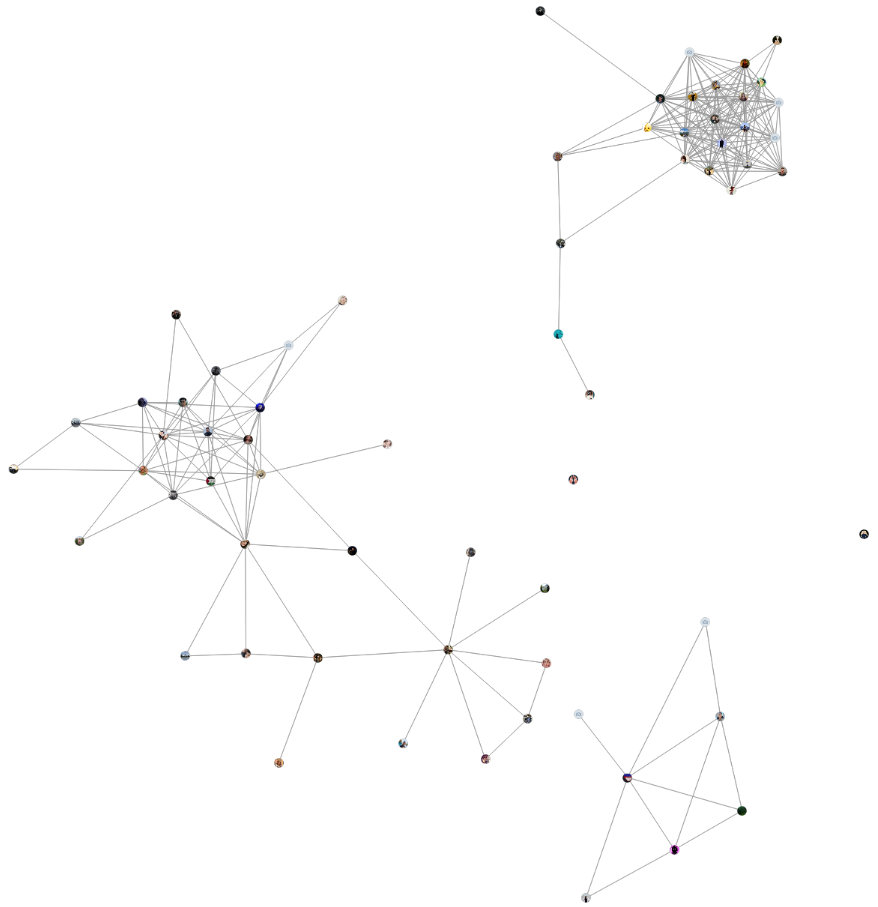
\includegraphics[width=.7\textwidth]{./imgs/fr.png}
  \end{minipage}
\caption{Результат визуализации с помощь алгоритма Фрюхтермана-Рейнгольда.}
\label{fig:fr_result}
\end{figure}


\begin{figure}[H]
\centering
  \begin{minipage}[t]{.9\textwidth}
  \centering
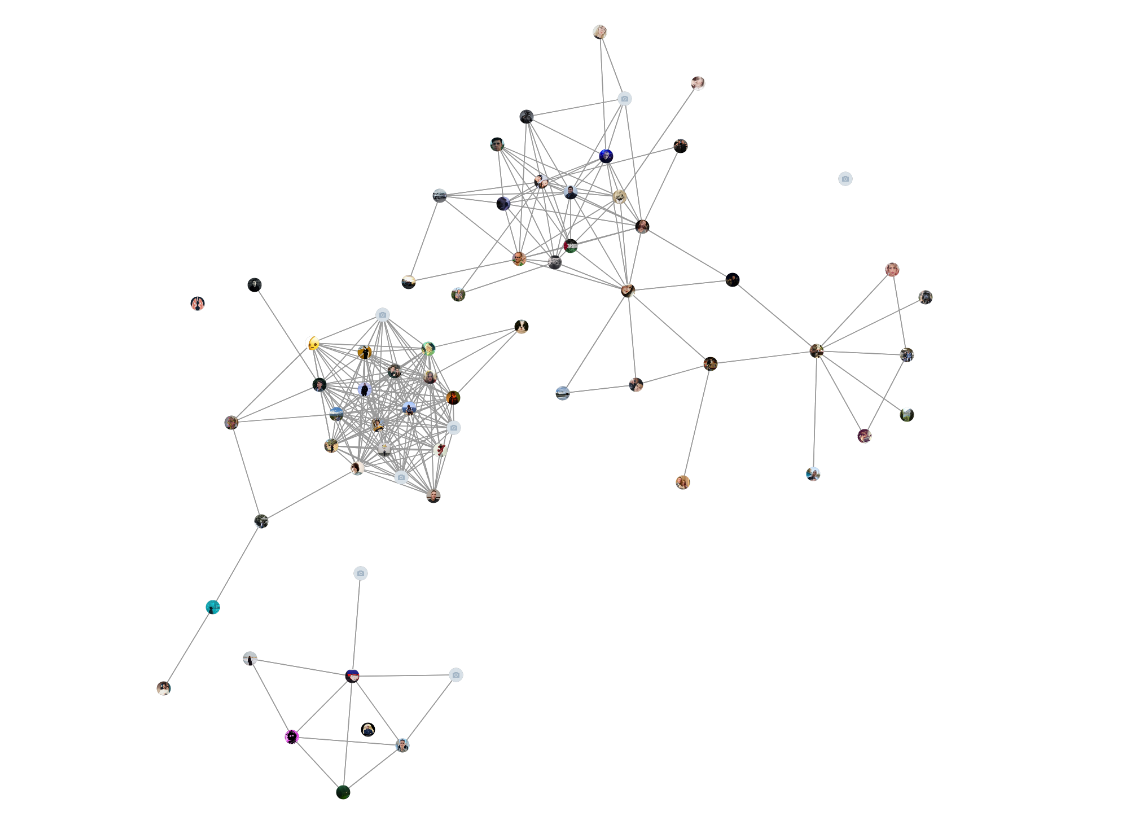
\includegraphics[width=.9\textwidth]{./imgs/kk.png}
  \end{minipage}
\caption{Результат визуализации с помощь алгоритма Камады-Кавай.}
\label{fig:kk_result}
\end{figure}

\section{Тестирование}

\newpage
\anonsection{ЗАКЛЮЧЕНИЕ}  %Заключение

\renewcommand\refname{СПИСОК ИСПОЛЬЗОВАННЫХ ИСТОЧНИКОВ}
% Список литературы
\clearpage
%\bibliographystyle{ugost2008s}  %utf8gost71u.bst} %utf8gost705u} %gost2008s}
{\catcode`"\active\def"{\relax}
\addcontentsline{toc}{section}{\protect\numberline{}\refname}%
%\bibliography{biblio} %здесь ничего не меняем, кроме, возможно, имени bib-файла
\printbibliography
}
\newpage
\settocdepth{section}
\anonsection{ПРИЛОЖЕНИЕ А}
\vspace{-30pt}




\begin{listing}[H]

    \caption{Модель двумерного вектора}
    \label{lst:vector_model}
    \inputminted[breaklines, frame=single,fontsize = \footnotesize, linenos, xleftmargin = 1.5em]{typescript}{./listings/vector.ts}
\end{listing}

\begin{listing}[H]
    \caption{Операции над векторами}
    \label{lst:vector_ops}
    \inputminted[breaklines, frame=single,fontsize = \footnotesize, linenos, xleftmargin = 1.5em]{typescript}{./listings/vector_ops.ts}
\end{listing}

\begin{listing}[H]
\caption{Модель пользователя}
\label{lst:user_model}
  \inputminted[frame=single,fontsize = \footnotesize, linenos, xleftmargin = 1.5em]{typescript}{./listings/user.ts}
\end{listing}

\begin{listing}
\caption{Модель вершины}
\label{lst:vertex_model}
  \inputminted[breaklines, frame=single,fontsize = \footnotesize, linenos, xleftmargin = 1.5em]{typescript}{./listings/vertex.ts}
\end{listing}

\begin{listing}
\caption{Модель графа}
\label{lst:graph_model}
  \inputminted[breaklines, frame=single,fontsize = \footnotesize, linenos, xleftmargin = 1.5em]{typescript}{./listings/graph.ts}
\end{listing}

\begin{listing}
\caption{Реализация класса VkAPI}
\label{lst:vkapi}
  \inputminted[breaklines, frame=single,fontsize = \footnotesize, linenos, xleftmargin = 1.5em]{typescript}{./listings/vkapi.ts}
\end{listing}

\begin{listing}
\caption{Структуры ответов}
\label{lst:responses}
  \inputminted[breaklines, frame=single,fontsize = \footnotesize, linenos, xleftmargin = 1.5em]{typescript}{./listings/responses.ts}
\end{listing}

\begin{listing}
\caption{Реализация алгоритма Фрюхтермана-Рейнгольда}
\label{lst:fr_alg}
  \inputminted[breaklines, frame=single,fontsize = \footnotesize, linenos, xleftmargin = 1.5em]{typescript}{./listings/fr.ts}
\end{listing}

\begin{listing}
\caption{Реализация функции нахождения отталкивающей силы}
\label{lst:rep_force}
  \inputminted[breaklines, frame=single,fontsize = \footnotesize, linenos, xleftmargin = 1.5em]{typescript}{./listings/rep.ts}
\end{listing}

\begin{listing}
\caption{Реализация функции нахождения притягивающей силы}
\label{lst:attr_force}
  \inputminted[breaklines, frame=single,fontsize = \footnotesize, linenos, xleftmargin = 1.5em]{typescript}{./listings/rep.ts}
\end{listing}


\begin{listing}
\caption{Реализация алгоритма Флойда-Уоршела}
\label{lst:fw_alg}
  \inputminted[breaklines, frame=single,fontsize = \footnotesize, linenos, xleftmargin = 1.5em]{typescript}{./listings/fw.ts}
\end{listing}


\begin{listing}
\caption{Метод поиска значения энергии вершины}
\label{lst:vertexen}
  \inputminted[breaklines, frame=single,fontsize = \footnotesize, linenos, xleftmargin = 1.5em]{typescript}{./listings/vertexen.ts}
\end{listing}

\begin{listing}
\caption{Метод поиска вершины с максимальным значением энергии}
\label{lst:maxen}
  \inputminted[breaklines, frame=single,fontsize = \footnotesize, linenos, xleftmargin = 1.5em]{typescript}{./listings/maxen.ts}
\end{listing}

\begin{listing}
\caption{Метод поиска нового положения вершины}
\label{lst:nextpos}
  \inputminted[breaklines, frame=single,fontsize = \footnotesize, linenos, xleftmargin = 1.5em]{typescript}{./listings/nextpos.ts}
\end{listing}

\begin{listing}
\caption{Реализация алгоритма Камады-Кавай}
\label{lst:kk_alg}
  \inputminted[breaklines, frame=single,fontsize = \footnotesize, linenos, xleftmargin = 1.5em]{typescript}{./listings/kk.ts}
\end{listing}

\begin{listing}
\caption{Реализация функции draw}
\label{lst:draw}
  \inputminted[breaklines, frame=single,fontsize = \footnotesize, linenos, xleftmargin = 1.5em]{typescript}{./listings/draw.ts}
\end{listing}



\end{document}
